\documentclass{article}

\usepackage{tgbonum}    % Tex Gyre Bonum
% \usepackage{mathptmx} % Times New Roman

% Header
\usepackage{fancyhdr}
\pagestyle{fancy}
\lhead{Daniel Jahn}
\rhead{Spatio-temporal clustering}
\cfoot{\thepage}
\renewcommand{\headrulewidth}{0.4pt}

% Images
\usepackage{graphicx}
\graphicspath{ {Images/} }

% Bibliography
\usepackage{natbib}
\bibliographystyle{unsrtnat}


% Todonotes
\usepackage{xargs} % For definining new todonotes
\usepackage[prependcaption,textsize=tiny]{todonotes} % disable
\newcommandx{\problem}[2][1=]{\todo[linecolor=red,backgroundcolor=red!25,bordercolor=red,#1]{#2}}
\newcommandx{\todoo}[2][1=]{\todo[linecolor=blue,backgroundcolor=blue!25,bordercolor=blue,#1]{#2}}
\newcommandx{\note}[2][1=]{\todo[linecolor=OliveGreen,backgroundcolor=OliveGreen!25,bordercolor=OliveGreen,#1]{#2}}
\newcommandx{\unsure}[2][1=]{\todo[linecolor=Plum,backgroundcolor=Plum!25,bordercolor=Plum,#1]{#2}}


% Mathematical symbols
\usepackage{amsmath}
\usepackage{amssymb}


% Options for the caption font
\usepackage[font=small]{caption}


\usepackage{titlesec}
\titleformat*{\subsection}{\normalsize\bfseries}

\begin{document}

% Article top matter
\title{NMST543 \\
Spatio-temporal clustering}
\author{Daniel Jahn \\
jahn@karlin.mff.cuni.cz}  
\date{\today} 
\maketitle

\tableofcontents


In this text, we investigate the spatio-temporal clustering method proposed in \cite{diggle1995}.

\section{Interaction and clustering}
In order to understand the term \textit{spatio-temporal clustering}, care has to be taken to carefully tease apart the related concepts of interaction and clustering, and then see how they transfer to the spatio-temporal case.


\textbf{Clustering}. Clustering typically refers to an a priori existing condition which affects the point process. We distinguish between spatial and temporal clustering. \textbf{Spatial clustering} results in the inhomogeneity of spatial distribution. An example is the crime rate being higher in densely populated areas. 
\textbf{Temporal clustering} results in the inhomogeneity of temporal distribution. An example are seasonal trends, such as an increased incidence of disease during winter. 
 
\textbf{Interaction} is typically understood to be a mechanism through which the location of one or more points influences the locations of others. For example, certain tree species prefer to grow further from other trees, thus resulting in repulsion between the individual locations. In the temporal domain, we have e.g. the refractory period for neurons, where one neuron remains inactive for a small period after firing. 

Both interaction and clustering result in inhomogeneity of the point patterns. From a statistical perspective, their difference is often purely interpretational, as they cannot distinguished through data only, but require domain knowledge to interpret the origin of the inhomogeneity. Furthermore, the distinction blurs even further in the spatio-temporal case, where different mixtures of spatial and temporal clustering and interaction are difficult to categorize. 
This is reflected by the fact that the terms clustering and interaction are used interchangeably in \cite{diggle1995}.

A mere presence of both spatial and temporal clustering do not suffice for spatio-temporal clustering. Events can cluster spatially in some location and also exhibit a periodic temporal trend, but unless these two trends interact, these events do not exhibit spatio-temporal clustering. 

A typical example is a contagious disease. Spatially, the incidence is higher in densely populated areas. Temporally, the disease could exhibit a repulsive behaviour, where an individual is unlikely to suffer from the same disease in succession. However, if the disease is contagious, we obtain a spatio-temporal interaction where the spatial and temporal components are no longer separable. It is precisely these kinds of inhomogeneities which \cite{diggle1995} investigate.



\section{Description of the method}
 Let $X$ be a \textbf{stationary} simple spatio-temporal point process on $\mathbb R^2\times \mathbb R$. We only observe the events $X\cap(W\times [0,T]),$ where $W$ is bounded Borel with $|W|>0$ and $T>0$. We define its projections to the spatial and temporal domain,
$$X_1 = \{x \in W: (x,t)\in X\cap (W\times [0,T])\}, \quad X_2 = \{t \in [0,T]: (x,t) \in X\cap (W\times [0,T])\},$$
and we assume $X_1$ and $X_2$ to be simple. We denote the intensity of $X$ by $\lambda$ and the intensities of $X_1$ and $X_2$ by $\lambda_1$ and $\lambda_2$, respectively. Note that $\lambda_1 = \lambda T$ and $\lambda_2 = \lambda |W|$.


We utilize the \textit{K-function}, which can be defined by
$$\lambda K(s,t) = \mathrm{E} \sum^{\neq}_{(x,t_1),(y,t_2)\in X} \frac{1_A(x) 1_{[0,s]}(\|x-y\|) 1_S(t_1) 1_{[0,t]}(|t_1 - t_2|)}{\lambda |A| |S|}$$
where $A \subset \mathbb R^2, S \subset \mathbb R$ are arbitrary Borel sets with finite and positive measure. We can interpret the term $\lambda K(s,t)$ as the number of further events occurring within distance $s$ and time $t$ of an arbitrary event.

Under the assumption of spatio-temporal independence, i.e. the independence of $X_1$ and $X_2$, we obtain the factorization
\begin{equation}\label{eq:h0}K(s,t)=K_1(s)K_2(t),\end{equation}
where $K_1$ and $K_2$ are the \todoo{Not really defined}K-functions of $X_1$ and $X_2$, respectively. Analogously, their interpretation is the number of further events occurring withing distance $s$, respectively within time $t$, of an arbitrary event.

The K-functions serve as a basis for the method proposed by \cite{diggle1995}. The functions $K,K_1,K_2$ will be used not only for testing for spatio-temporal interaction, but also to measure the extent and nature of it.

\subsection{Estimates}

Let $\{(x_i,t_i): i=1,\dots, n\}$ denote the locations and times of all events within $W\times [0,T]$. We introduce the estimates
$$\hat K(s,t) = |A|T (n(n-1))^{-1} \sum_{j\neq i} w_{ij} v_{ij} I_{[d_{ij} \leq s]} I_{[u_{ij} \leq t]},$$	
$$\hat K_1(s) = |A| (n(n-1))^{-1} \sum_{j\neq i} w_{ij}  I_{[d_{ij} \leq s]},$$	
$$\hat K_2(t) = T (n(n-1))^{-1} \sum_{j\neq i}  v_{ij}  I_{[u_{ij} \leq t]},$$
where $d_{ij} = \|x_i - x_j\|$ and $u_{ij} = |t_i - t_j|$, and $w_{ij}$ and $v_{ij}$ are edge-effect corrections.


We now introduce the three visual diagnostics which can be used to describe the extent and nature of the spatio-temporal interaction.

\subsection{Diagnostic surface plot}
Define a diagnostic function

$$\hat D(s,t) = \hat K(s,t) - \hat K_1(s) \hat K_2(t),$$

which should, under the null hypothesis, approximately equal to zero thanks to \eqref{eq:h0}. The value of $\hat D(s,t)$ is proportional to the increase of events compared to a process with the same spatial and temporal structure, but no spatio-temporal interaction. A surface plot of this function reveals the areas where the analyzed process differs from the null hypothesis.




\subsection{Residual plot}
The idea of residual analysis for point patterns has only been widely introduced quite recently (\cite{Baddeley2005}). However, \cite{diggle1995} already introduces a variant of it. 

To standardize the values of $\hat D(s,t)$, we can use the variance $V(s,t) = \mathrm{var} \hat D(s,t)$, where the variance is taken with respect to a random permutation of the times, while letting the locations be fixed. 

We can then introduce the residual function

$$R(s,t) = \hat D(s,t)/ \sqrt{V(s,t)}.$$ 

The plot of $R(s,t)$ against $\hat K_0(s,t) := \hat K_1(s) \hat K_2(t)$ is then an analogue of standardized residuals in regression modelling. In practice, $\sqrt{V(s,t)}$ is replaced by the empirical standard error of $D(s,t)$.


\subsection{Monte-Carlo test}
Although the distributions of the quantities introduced a generally intractable, we can still devise a statistical test using the Monte-Carlo methods.

Under the null hypothesis, we can obtain sampling distributions by letting the locations be fixed and randomly permuting the times, or vice versa. The values of $\hat D(s,t)$ could be used, but since $\hat K_1(s)$ and $\hat K_2(t)$ remain unchanged under the permutations, we only need to consider the values of 
$$Q(s,t) = \sum_{j\neq i} w_{ij} v_{ij} I_{[d_{ij} \leq s]} I_{[u_{ij} \leq t]}.$$

To devise a global test, one might use a discrete approximation to the integral of the standardized residual surface,
$$U=\sum_s \sum_t R(s,t).$$ 

The histogram of values of $U$ for the permuted point patterns together with the observed value constitute the second diagnostic visualisation. Furthermore, in a standard Monte-Carlo procedure, the values can be ranked to obtain a formal test.






\section{Implementation}
The methods from \cite{diggle1995} were implemented in \texttt{R} in the package \texttt{splancs}. The function \texttt{stkhat} provides an estimate of $\hat K(s,t), \hat K_1(s)$ and $\hat K_2(t)$. The standard error of $\hat D(s,t)$ is proved by \texttt{stsecal}. The permutation test, as well as values of the test statistic, can be obtained by \texttt{stmctest}, though the function uses the non-standardized test statistic
$$\sum_s \sum_t D(s,t)$$
instead.
Finally, the function \texttt{stdiagn} provides the three diagnostic visualisations introduced in the previous section, as well as a visualisation of $X_1$. This function produced the figures in this text.


\section{Simulated data}

Three types of models were simulated to investigate the method. The observation window is $[0,1]^3$ for all the models.

\subsection{Poisson process}

The first is the Poisson process, representing complete spatial randomness. Figure \ref{fig:poissonPP} contains one realization and Figure \ref{fig:poissonDiag} contains the diagnostic plots. The residual plot shows a surprisingly large residuals. Subsequent simulations showed that this behaviour is common. Although the residuals seem to suggest a trend, this is most likely simply because of the cumulative nature of the K-function. The plot of the function $D(s,t)$ shows a small scale of deviations from the null hypothesis, similarly to MC test plot.


\subsection{Thomas process}
The second is the Thomas process, an example of a clustering point process. Thomas process is a Poisson cluster process where the daughter distribution is a 3-dimensional normal distribution, $N_3(0,\sigma^2 I)$. Two realizations were simulated. 

The first, depicted in Figure \ref{fig:thomasPP} and diagnostic plots in Figure \ref{fig:thomasDiag}, has fewer parent points (intensity 20) and less dispersed clusters ($\sigma^2 = 0.02$). The residual plot and MC histogram clearly suggest a positive interaction. The plot of $D(s,t)$ shows a local maximum at the scale of the width of the clusters, but higher peaks can be found at the inter-cluster distance. The residual plot also shows large variance for values of $K_0(s,t)$ close to zero, which is a behaviour shared by virtually every realization of every model.

The second realization, depicted in Figures \ref{fig:thomas2PP} and  \ref{fig:thomas2Diag}, had more parent points (intensity 40), less points per cluster (intensity 20) and a higher cluster width ($\sigma^2=0.05$). The effects are now less pronounced, yet still clear. Interestingly, the plot of $D(s,t)$ show that the function attains negative values at larger distances, a behaviour that is nevertheless quite possible under clustering.


\subsection{Mat\'{e}rn process}

The last is the Mat\'{e}rn type II process, an example of a point process with a repulsive interaction. In Mat\'{e}rn type I process, a Poisson point process is simulated any two points closer (in the 3-dimensional Euclidean distance) than some threshold $r>0$ are removed. Only one randomly chosen point is removed for Mat\'{e}rn type II process. Two realizations with $r=0.05$ (Figures  \ref{fig:maternPP} and \ref{fig:maternDiag}) and $r=0.1$ (Figures  \ref{fig:matern2PP} and \ref{fig:matern2Diag}) were simulated.

They both show minimal deviations from the null hypothesis, suggesting that the method perhaps only detects a clustering behaviour and not repulsive interaction. Indeed the visual aids suggest a lesser deviation from the null hypothesis than in the case of the Poisson process. The only indication of a repulsive behaviour is perhaps the negative value of the observed statistic in the MC results plot.



\begin{figure}[p]
  \centering
    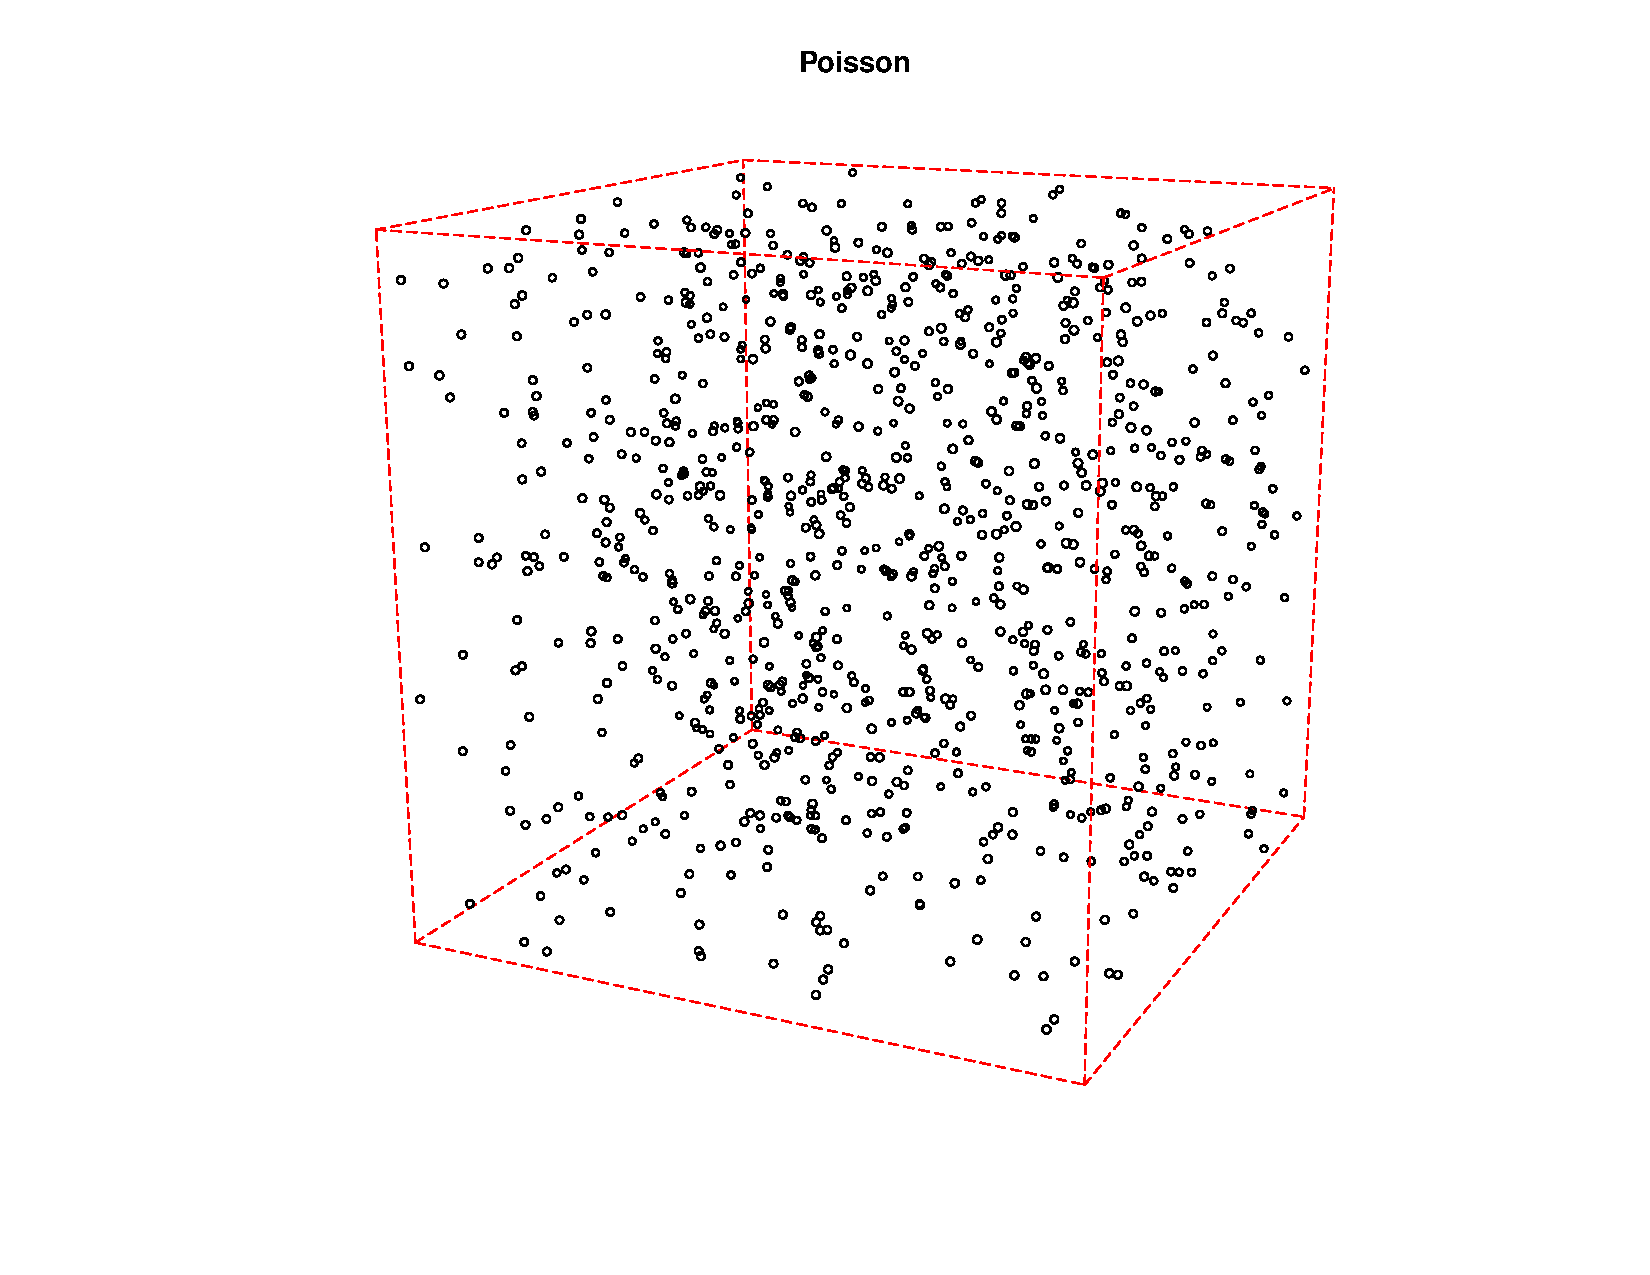
\includegraphics[width=0.9\textwidth]{PP_Poisson_1000_978.pdf}
  \caption{Realization of a Poisson point process. Intensity . Number of points: 978}
  \label{fig:poissonPP}


	\vspace*{\floatsep}

    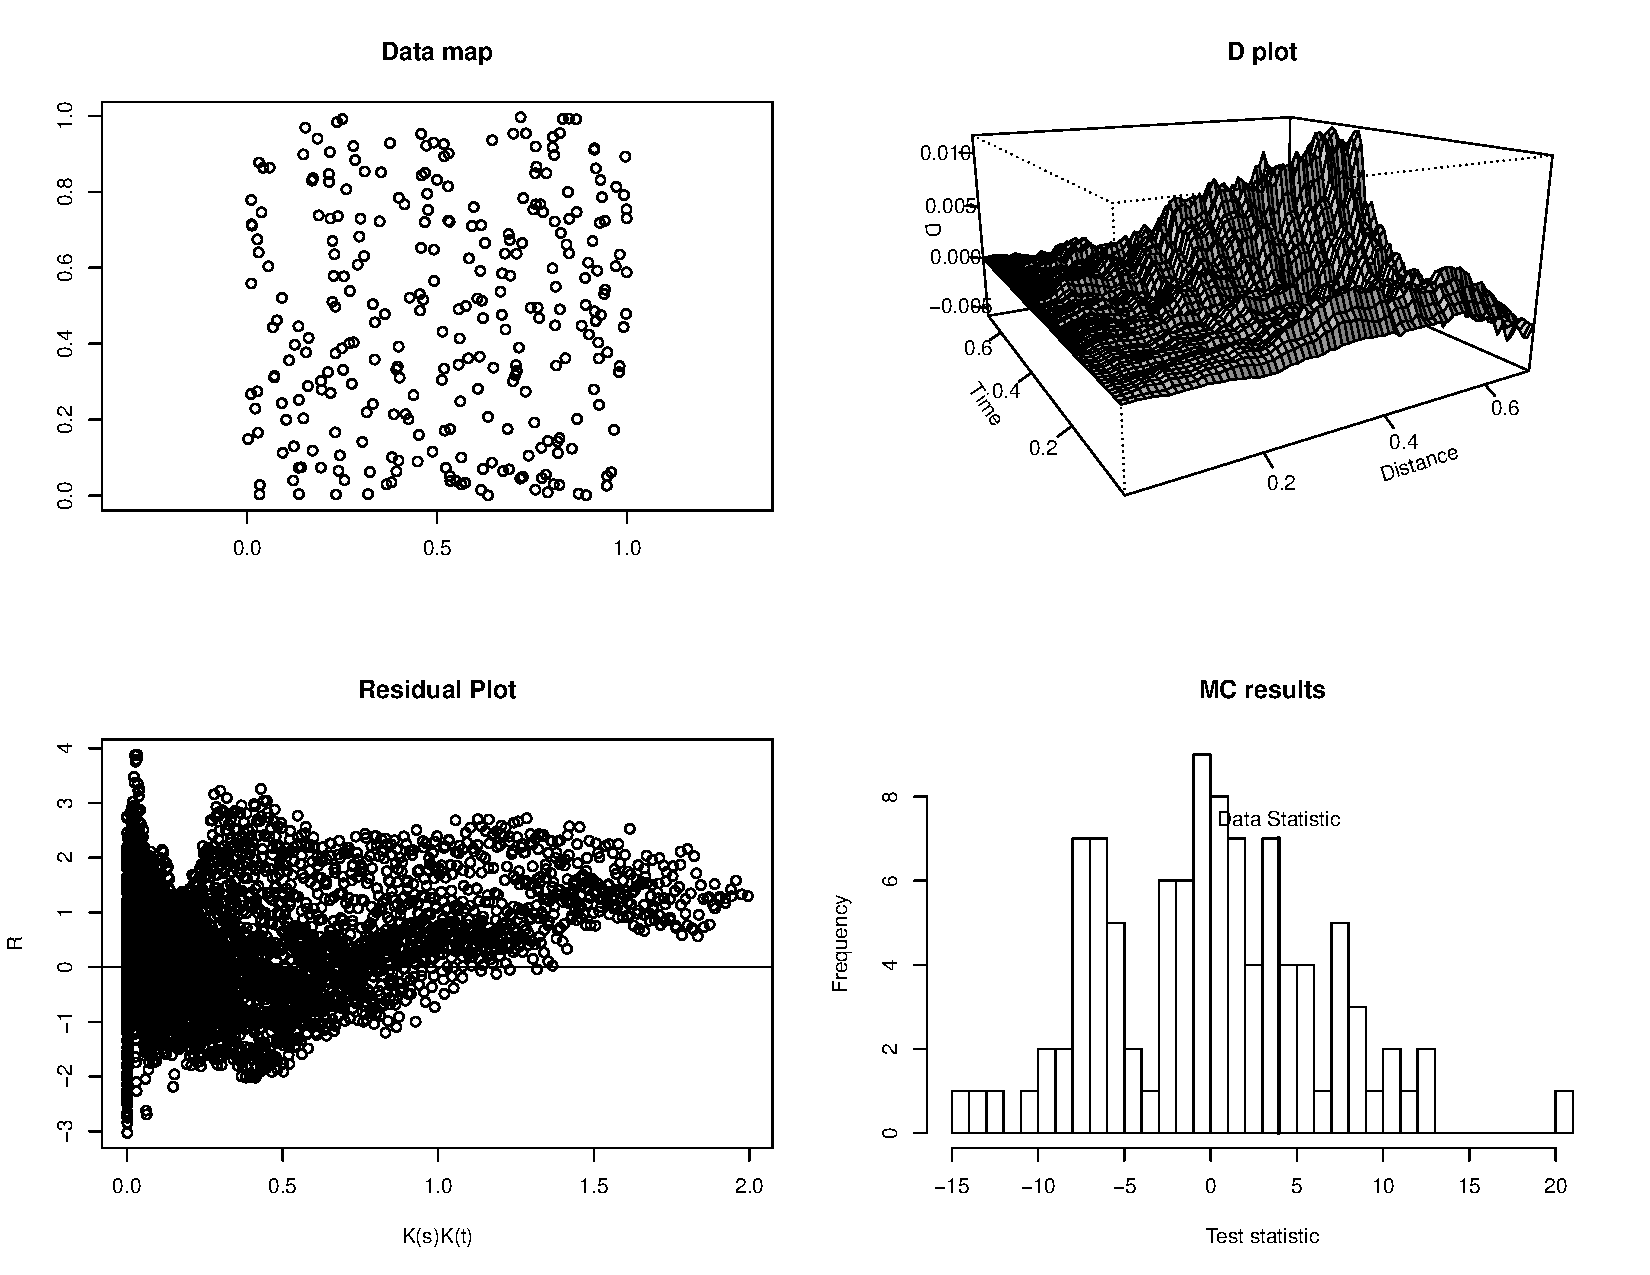
\includegraphics[width=0.9\textwidth]{diag_Poisson_1000_978.pdf}
  \caption{Diagnostic plots for a realization of a Poisson point process. Intensity . Number of points: 978}
  \label{fig:poissonDiag}
\end{figure}


\begin{figure}[p]
  \centering
    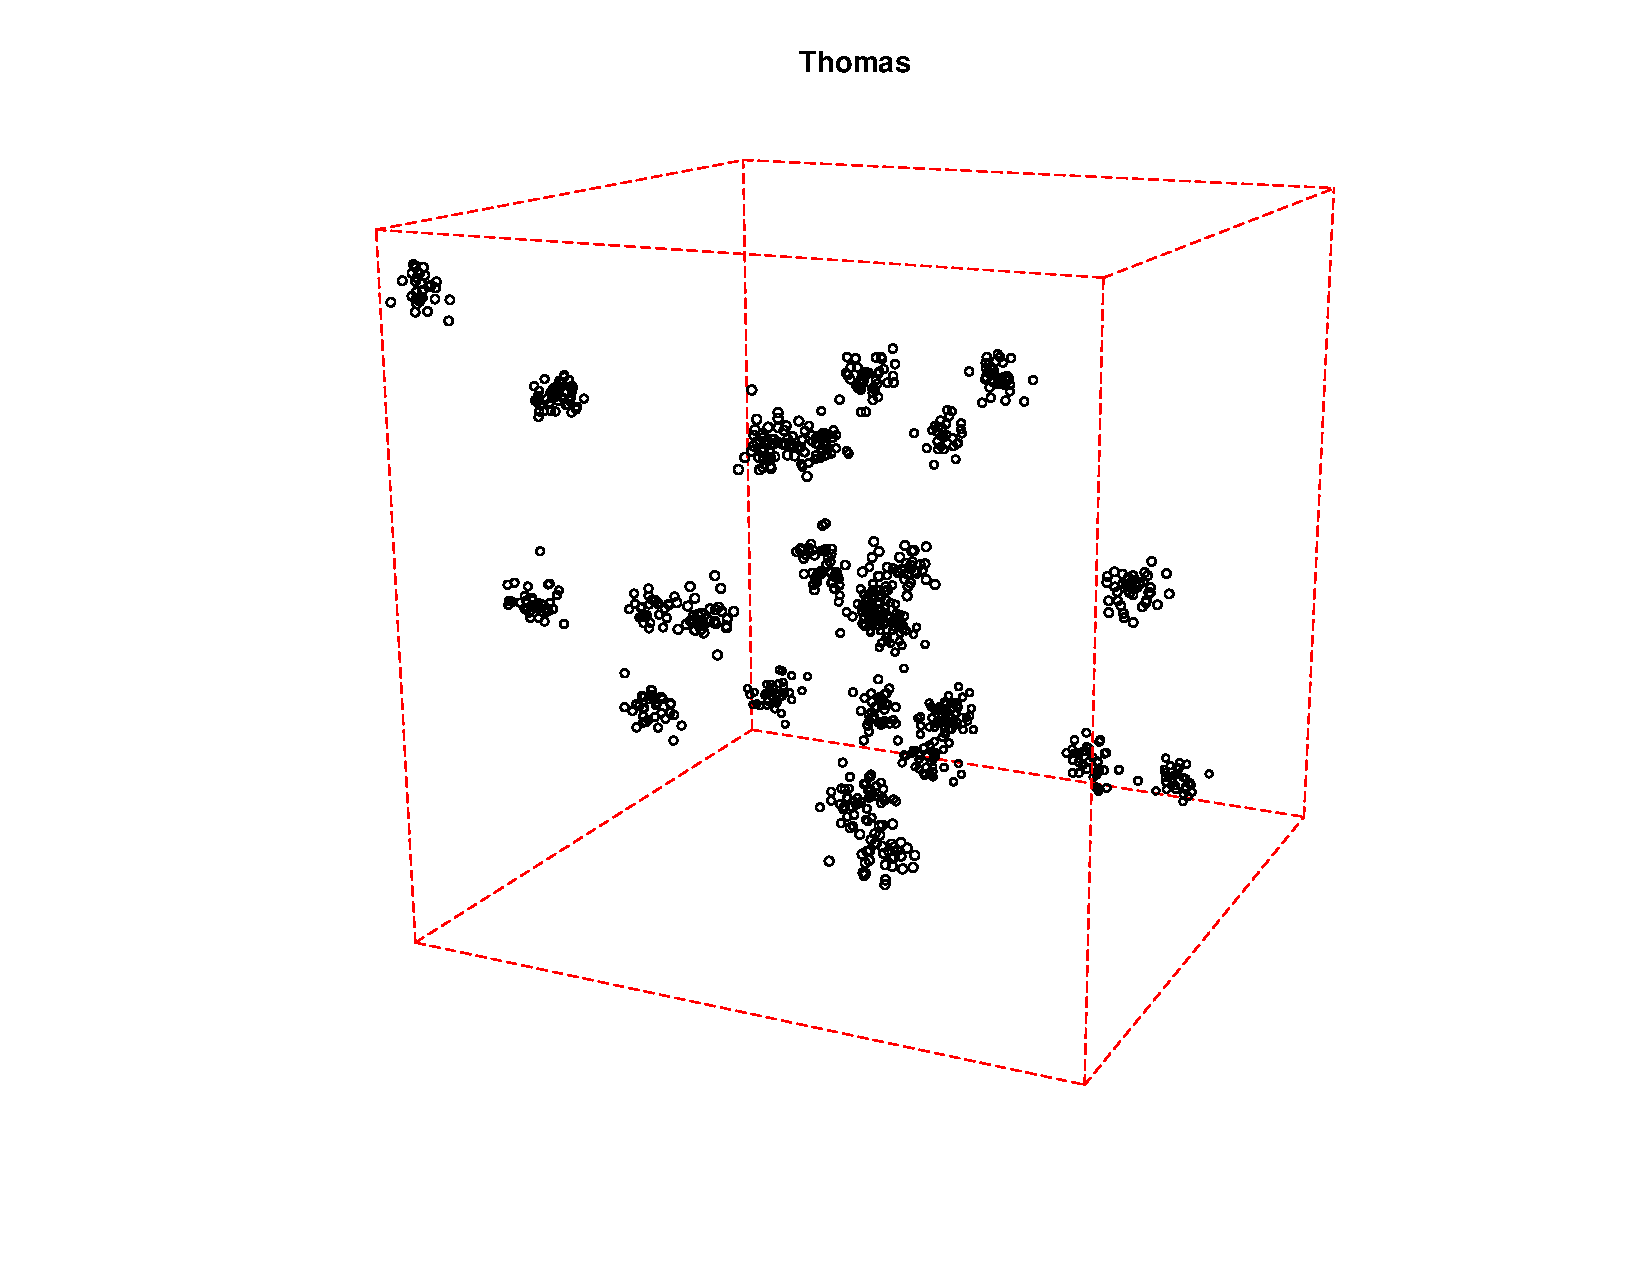
\includegraphics[width=0.9\textwidth]{PP_Thomas_20_40_0p02_949.pdf}
  \caption{Realization of a Thomas point process. Intensity of parent process 20. Daughter process: intensity 40, distribution $N(0,0.02)$. Number of points: 949.}
  \label{fig:thomasPP}

\vspace*{\floatsep}

    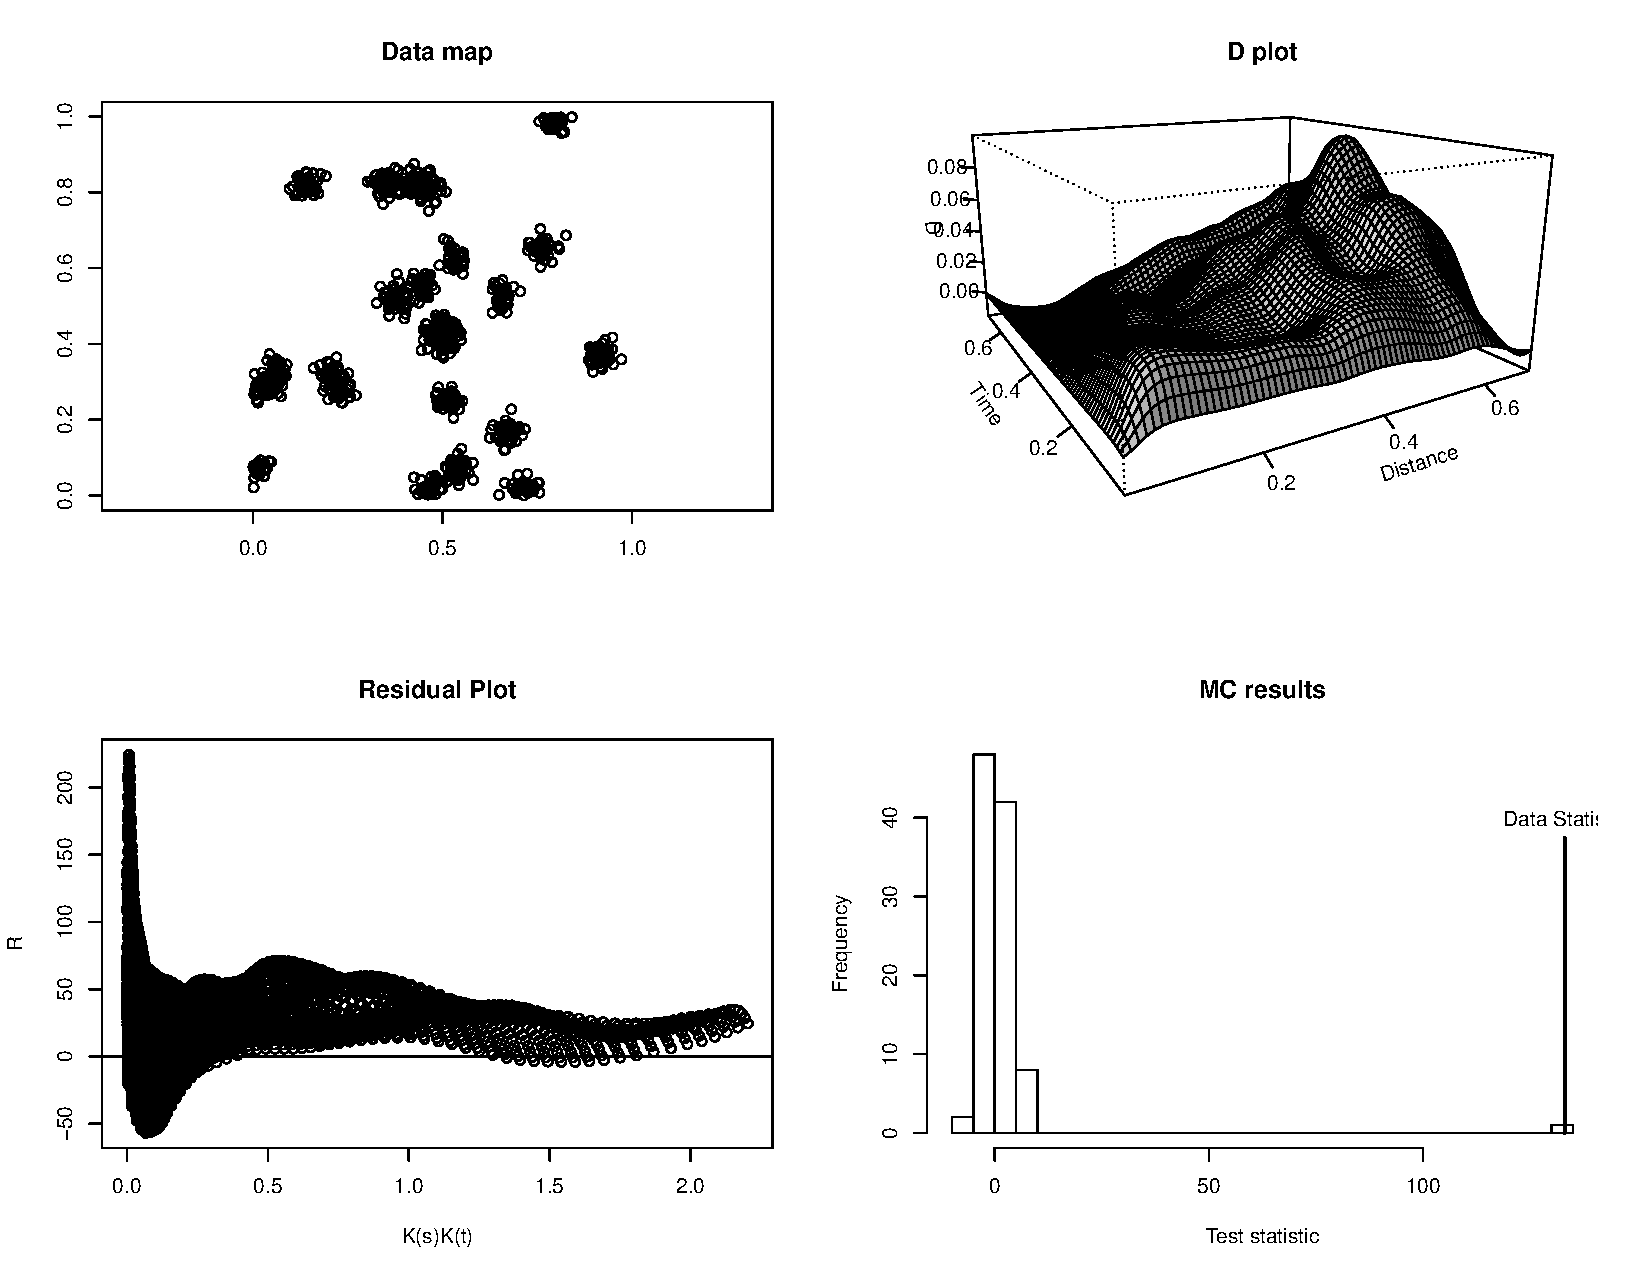
\includegraphics[width=0.9\textwidth]{diag_Thomas_20_40_0p02_949.pdf}
  \caption{Diagnostic plots for a realization of a Thomas point process. Intensity of parent process 20. Daughter process: intensity 40, distribution $N(0,0.02)$. Number of points: 949.}
  \label{fig:thomasDiag}
\end{figure}


\begin{figure}[p]
  \centering
    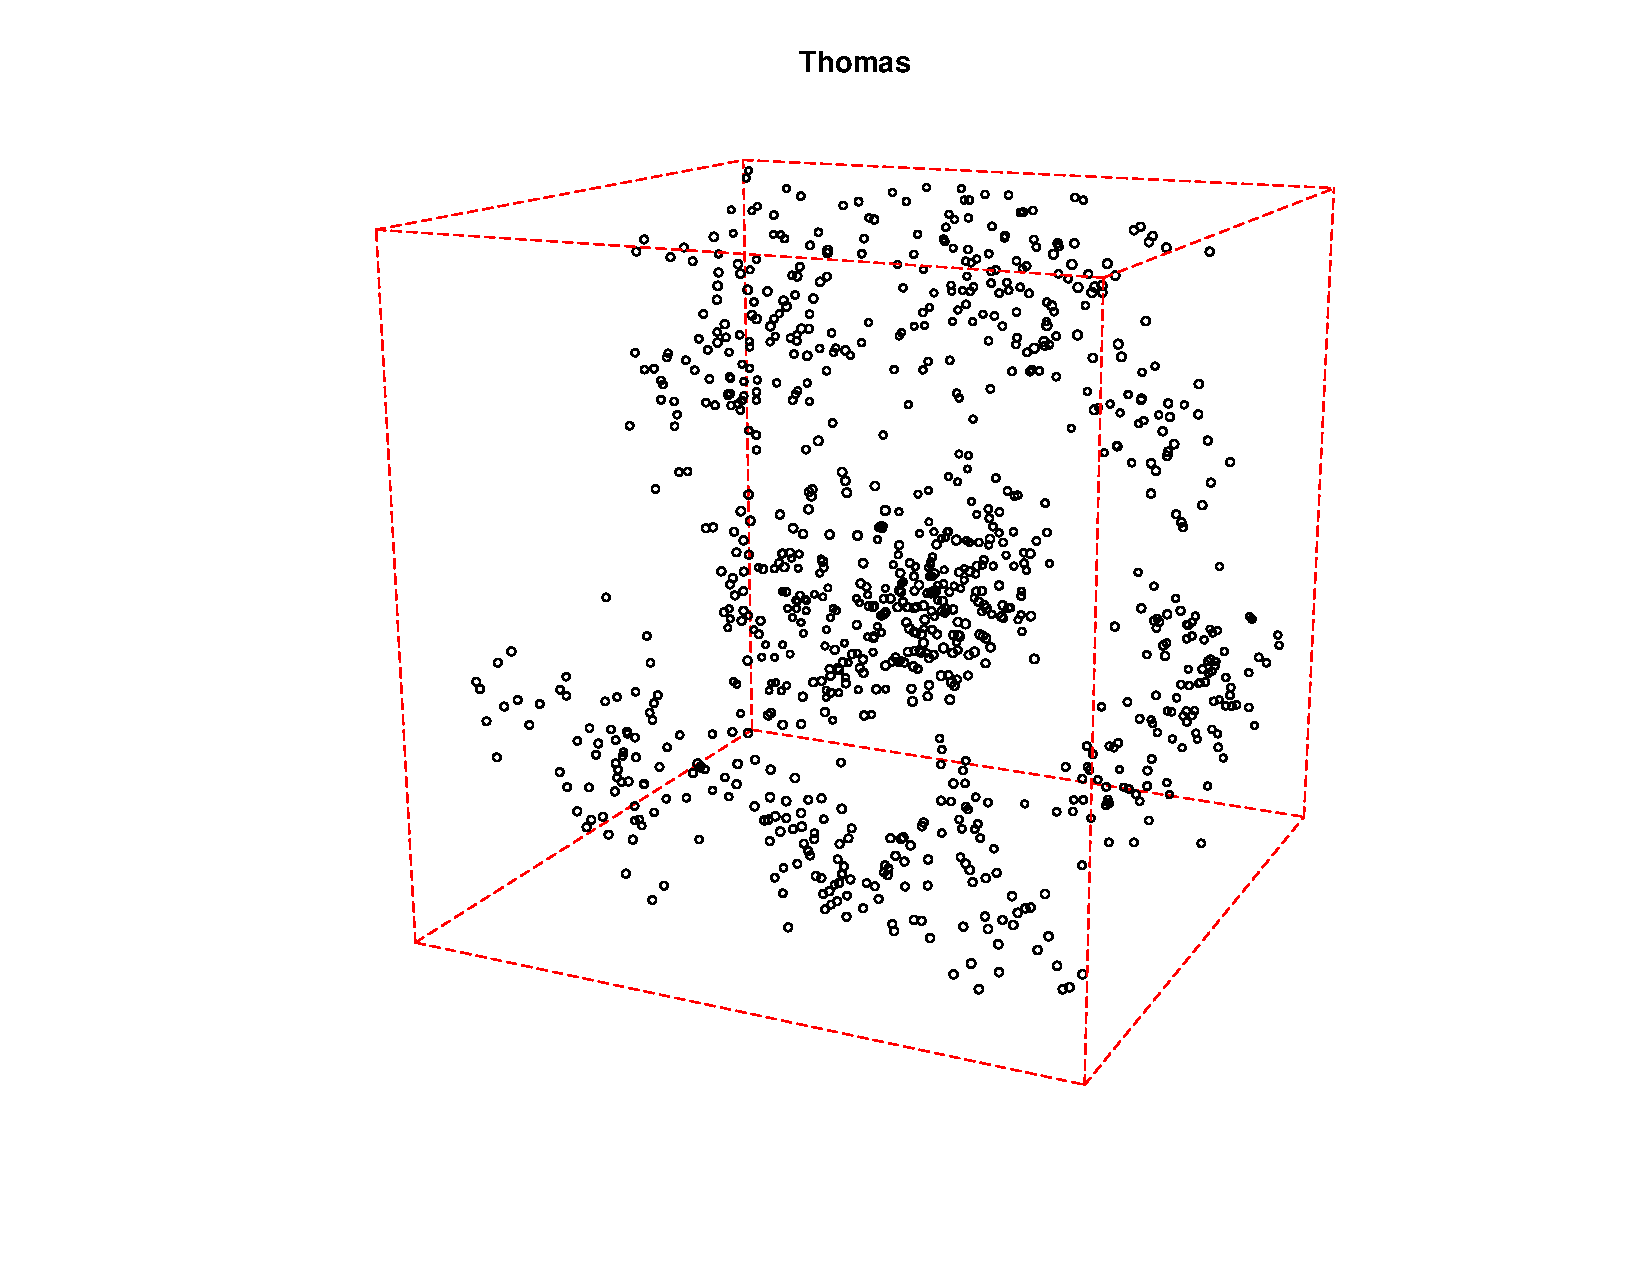
\includegraphics[width=0.9\textwidth]{PP_Thomas_40_20_0p05_929.pdf}
  \caption{Realization of a Thomas point process. Intensity of parent process 40. Daughter process: intensity 20, distribution $N(0,0.05)$. Number of points: 929.}
  \label{fig:thomas2PP}

\vspace*{\floatsep}

    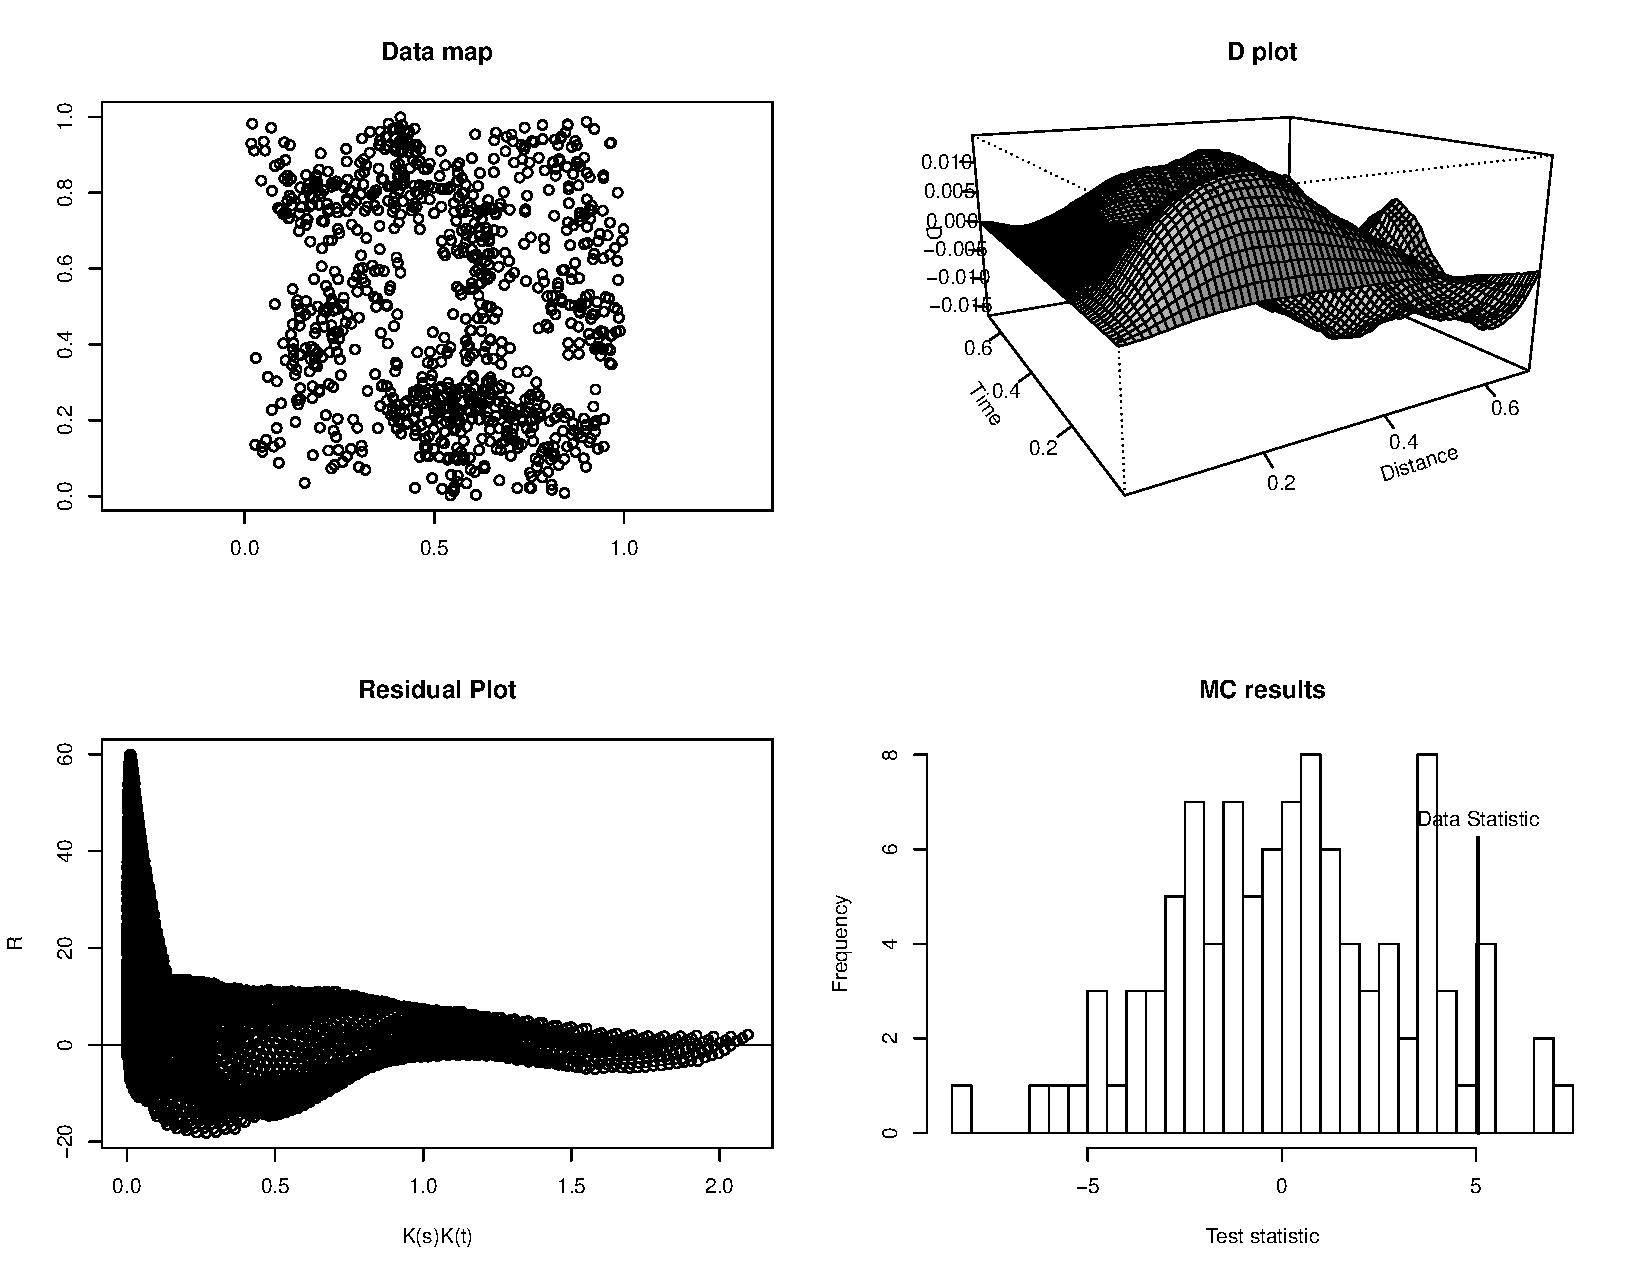
\includegraphics[width=0.9\textwidth]{diag_Thomas_40_20_0p05_929.pdf}
  \caption{Diagnostic plots for a realization of a Thomas point process. Intensity of parent process 40. Daughter process: intensity 20, distribution $N(0,0.05)$. Number of points: 929.}
  \label{fig:thomas2Diag}
\end{figure}



\begin{figure}[p]
  \centering
    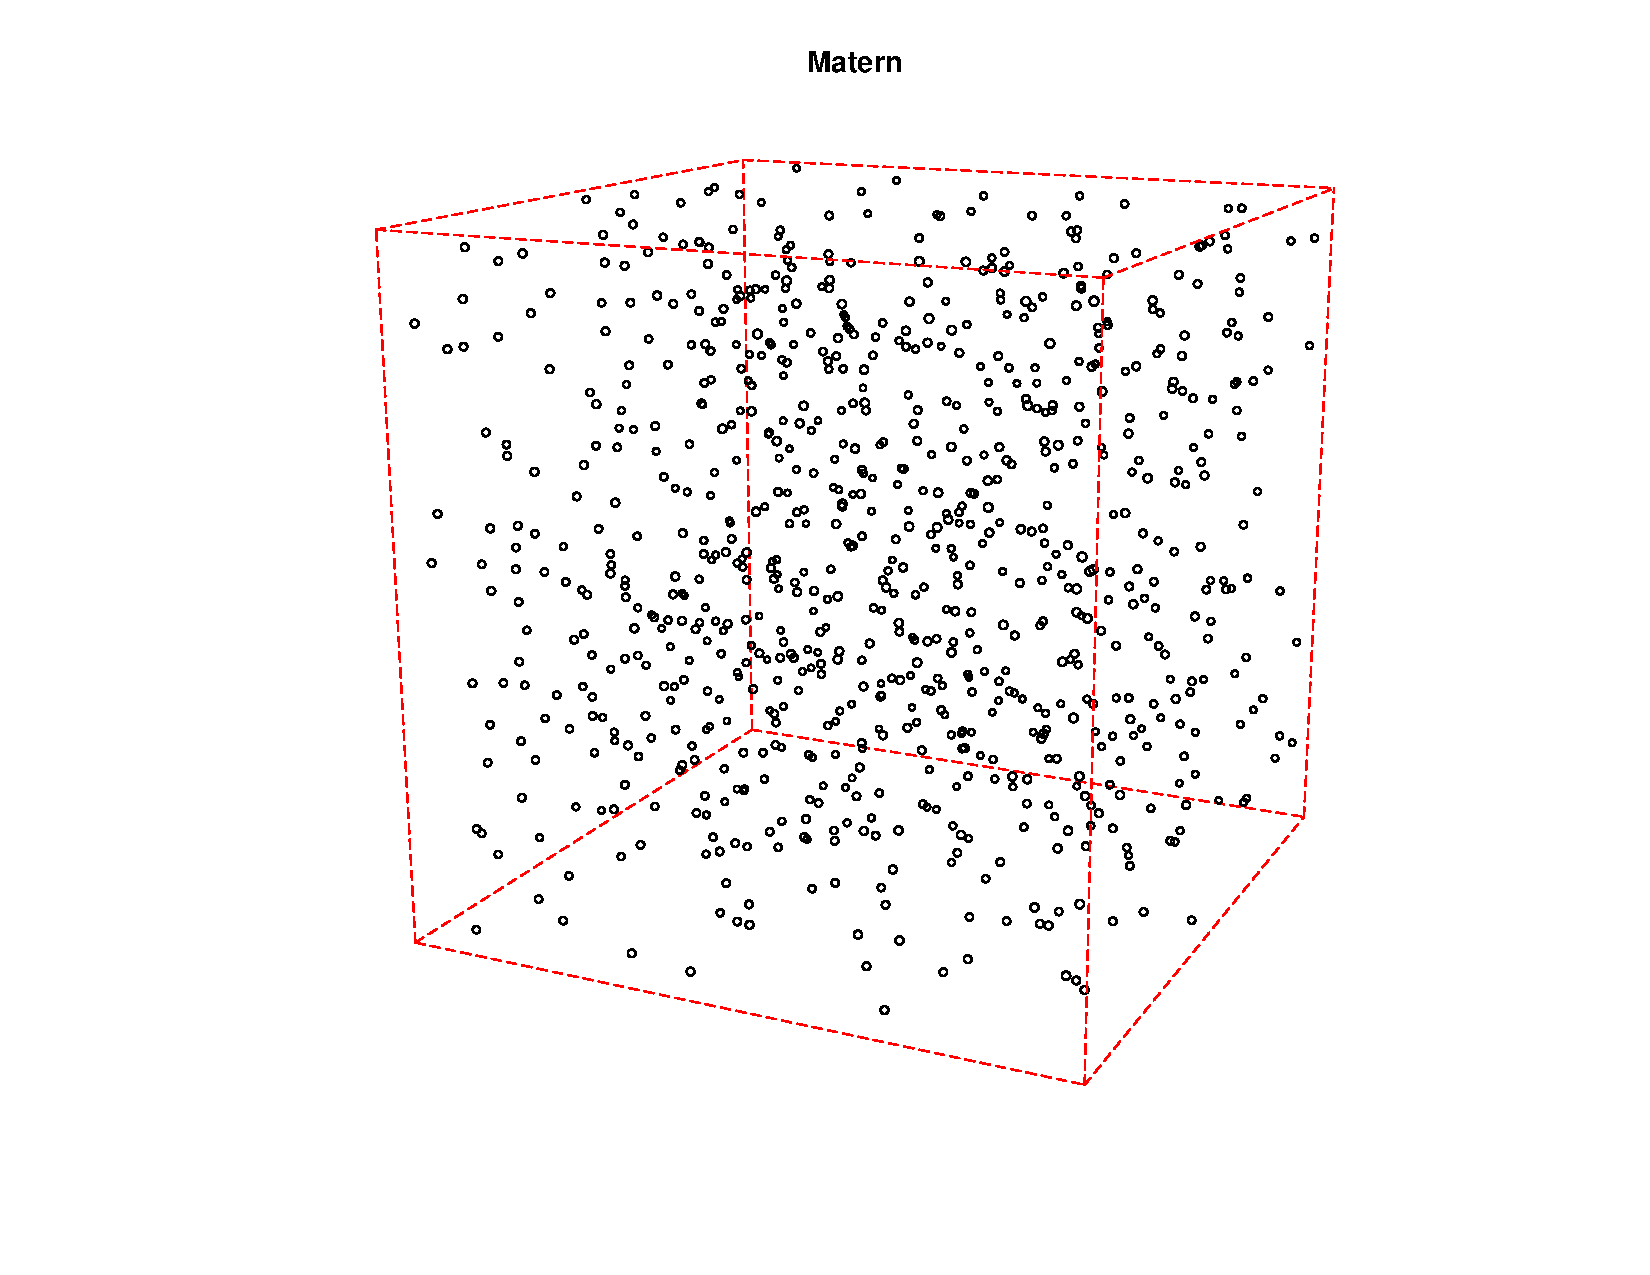
\includegraphics[width=0.9\textwidth]{PP_Matern_II_1000_0p05_818.pdf}
  \caption{Realization of a Matern II point process. Intensity 1000. Minimum distance 0.05. Number of points: 818.}
  \label{fig:maternPP}

\vspace*{\floatsep}

    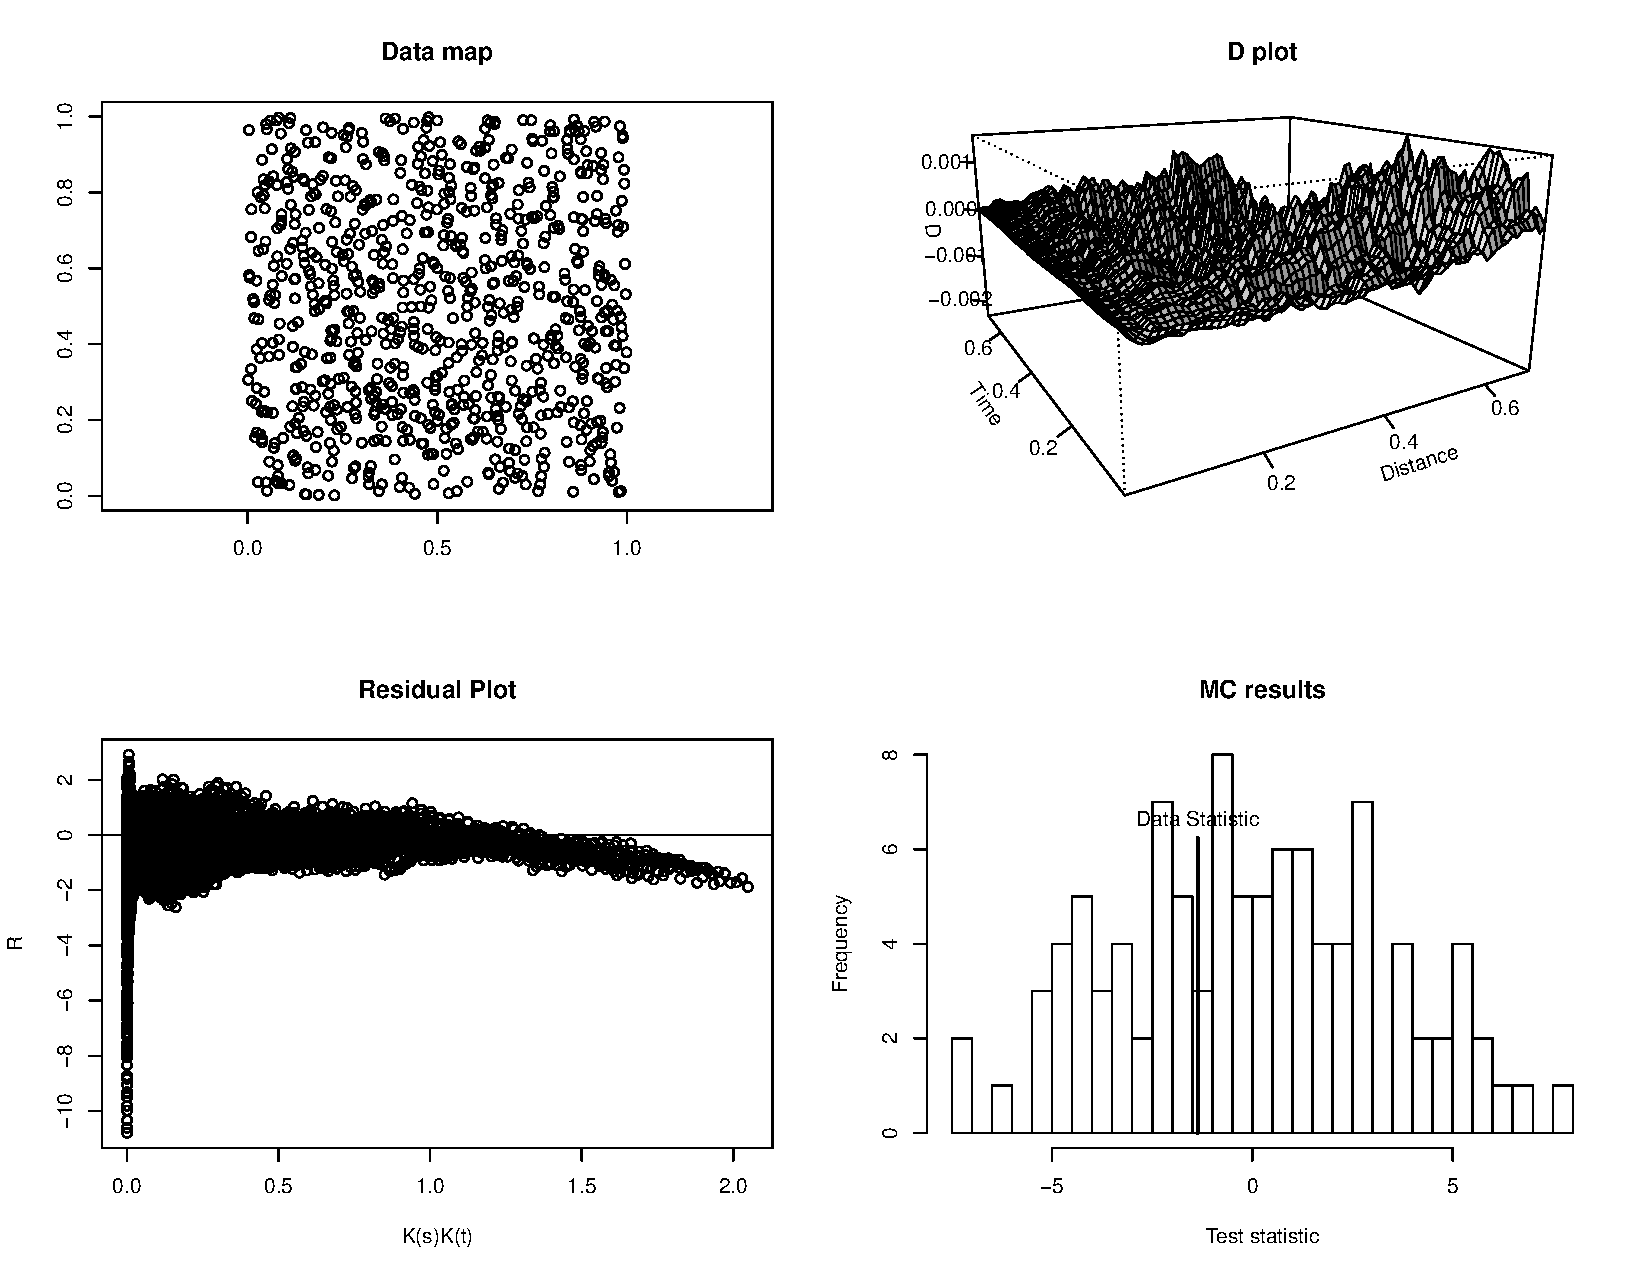
\includegraphics[width=0.9\textwidth]{diag_Matern_II_1000_0p05_818.pdf}
  \caption{Diagnostic plots for a realization of a Matern II point process.  Intensity 1000. Minimum distance 0.05. Number of points: 818.}
  \label{fig:maternDiag}
\end{figure}




\begin{figure}[p]
  \centering
    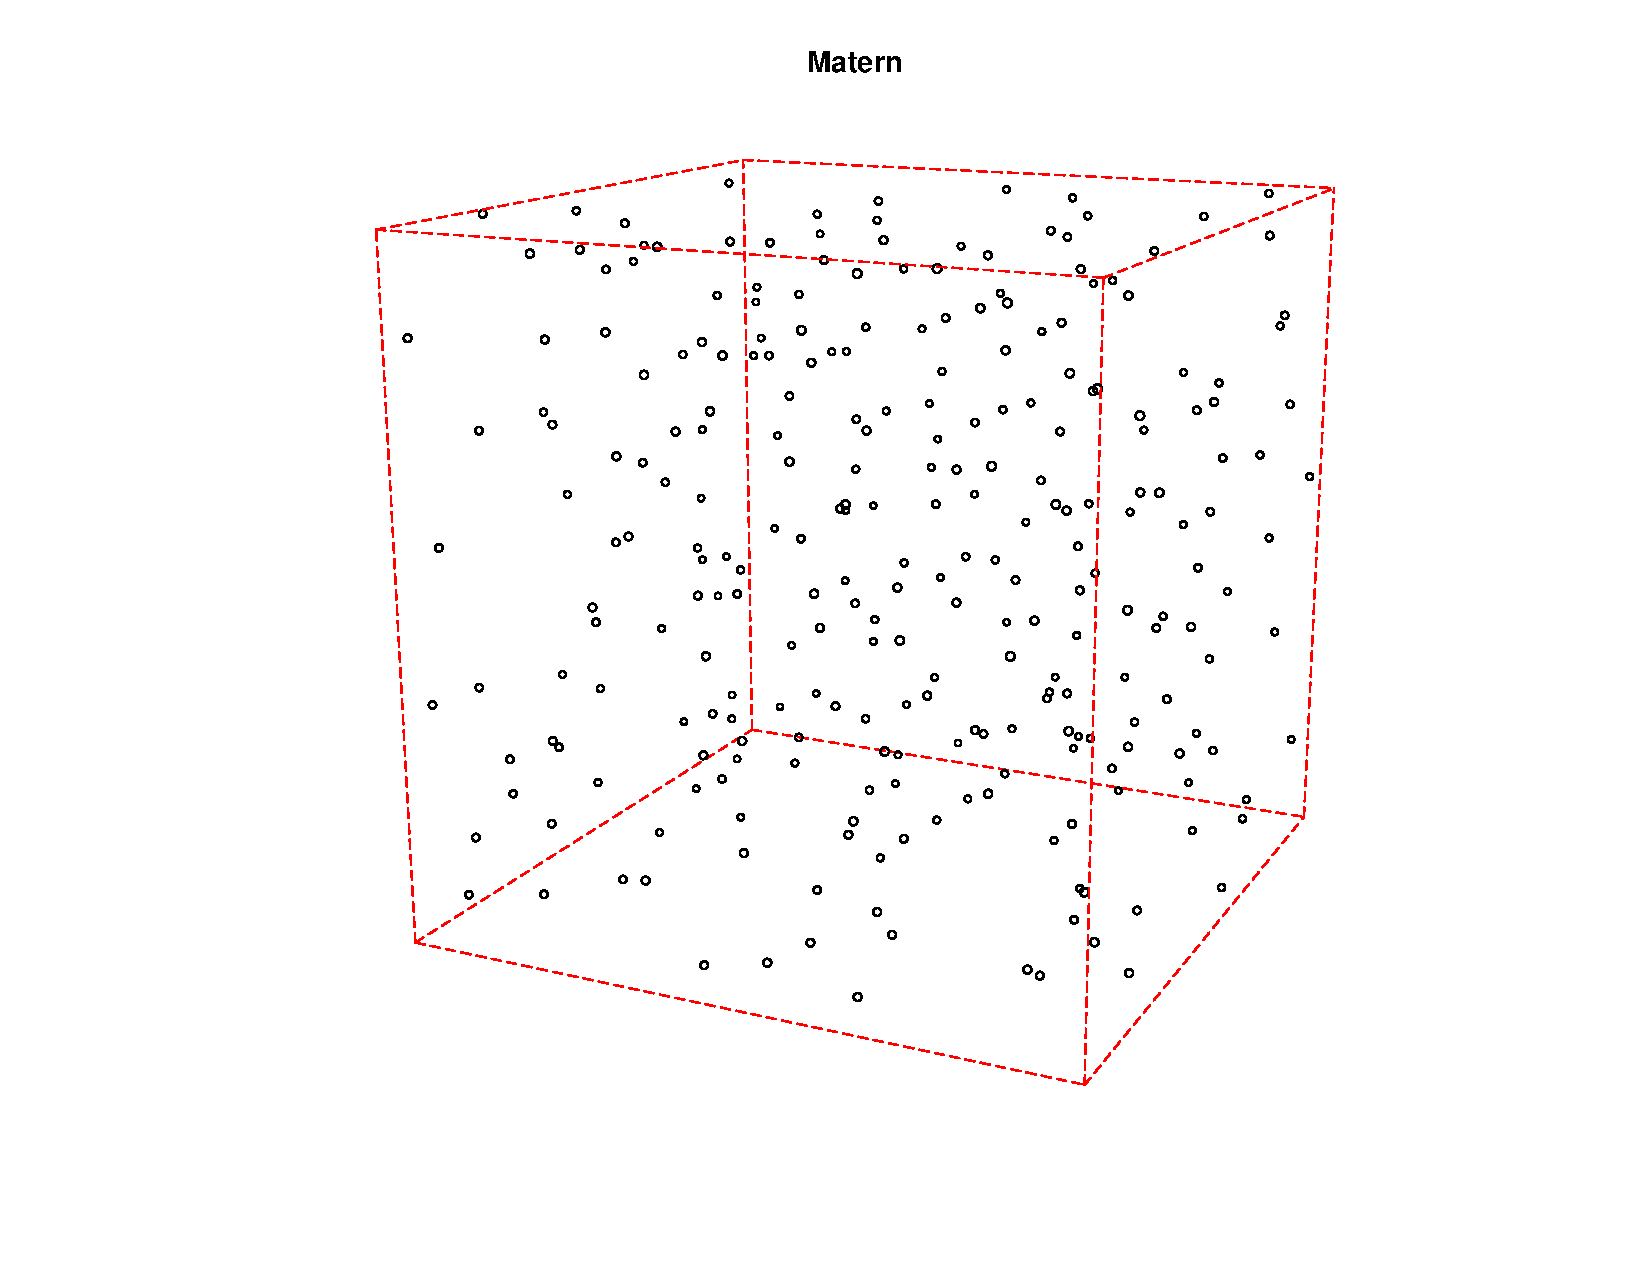
\includegraphics[width=0.9\textwidth]{PP_Matern_II_1000_0p1_275.pdf}
  \caption{Realization of a Matern II point process. Intensity 1000. Minimum distance 0.1. Number of points: 275.}
  \label{fig:matern2PP}

\vspace*{\floatsep}

    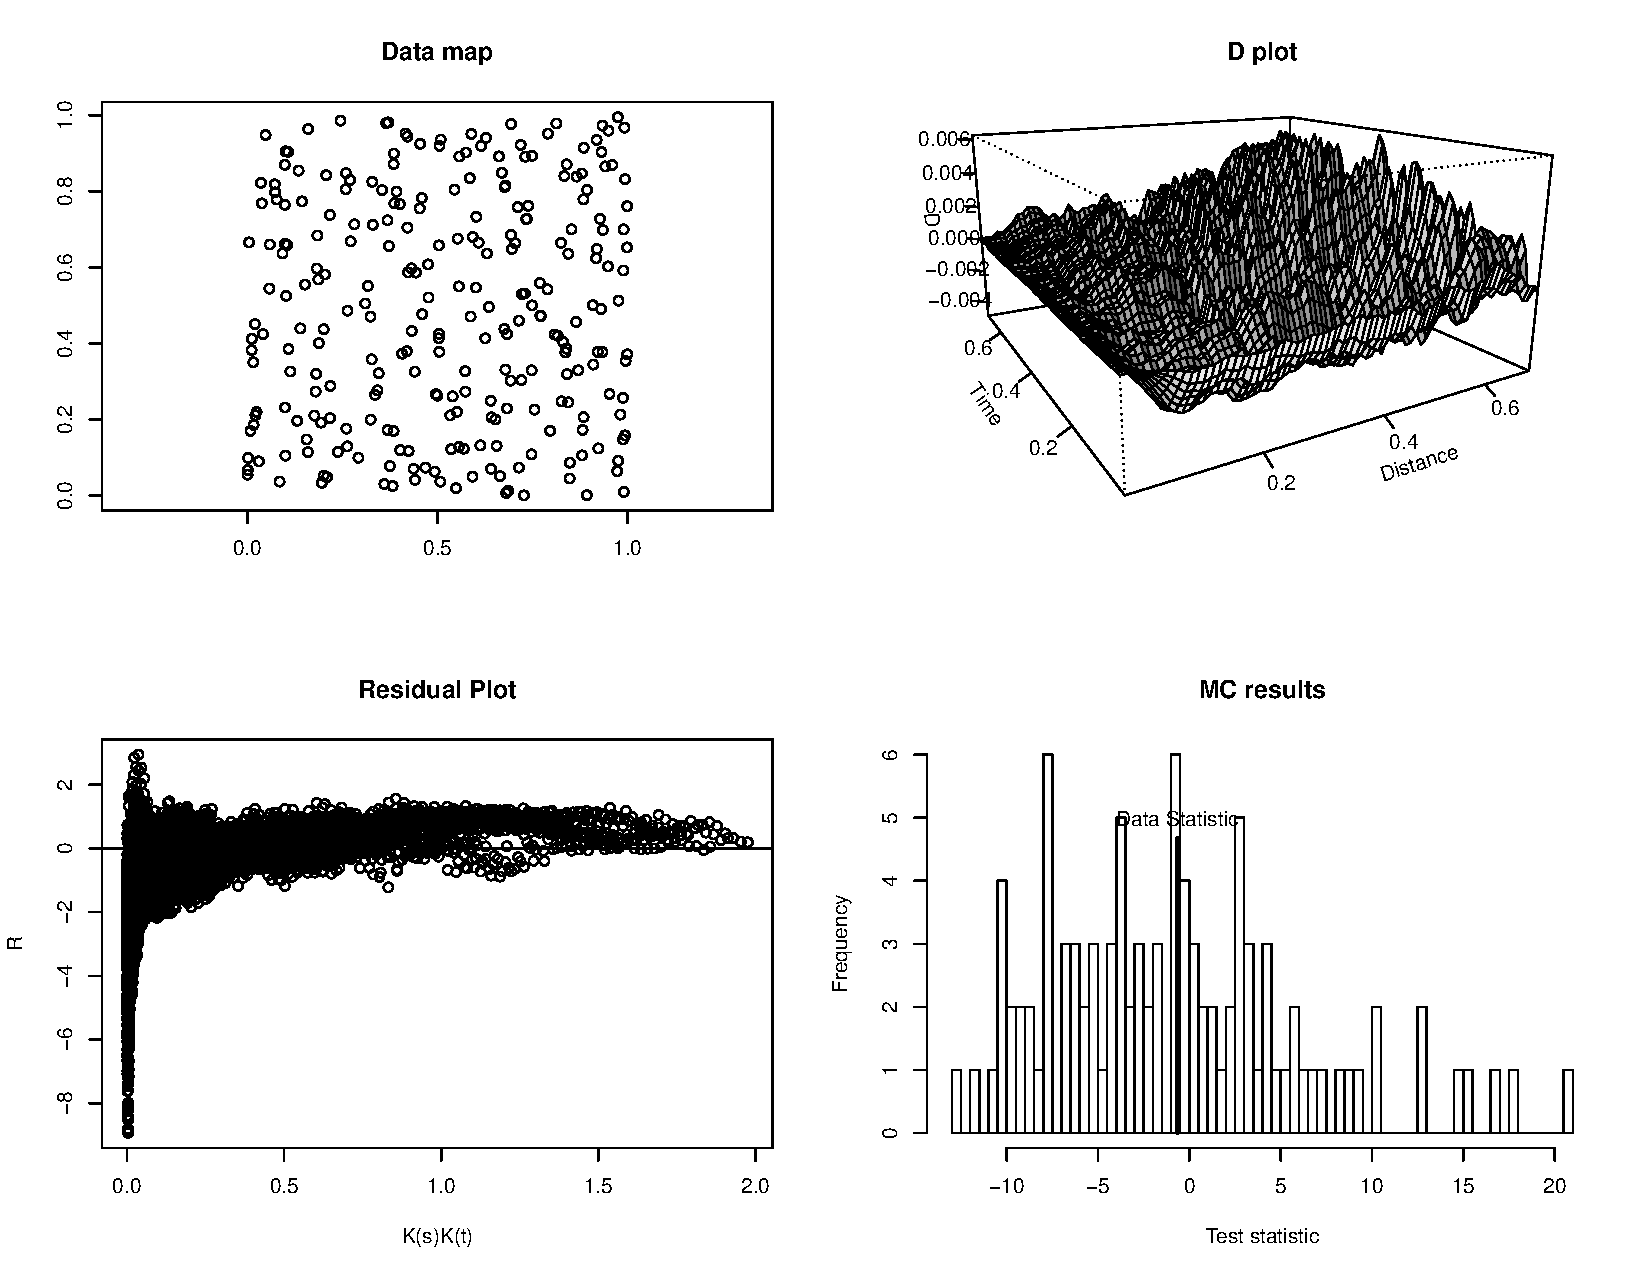
\includegraphics[width=0.9\textwidth]{diag_Matern_II_1000_0p1_275.pdf}
  \caption{Diagnostic plots for a realization of a Matern II point process.  Intensity 1000. Minimum distance 0.1. Number of points: 275.}
  \label{fig:matern2Diag}
\end{figure}





\section{Real data}
The real dataset consists of data about flat occupancy in one neighborhood in Baltimore throughout 11 years. A point at $(s,t)$ means that a flat at location $s$ was vacant during the year $t$. The data was standardized to fit the observation window $[0,1]^3$. 

This dataset has a number of features which test the limitations of this approach. The projected point patterns are not simple, as the same flat can be vacant throughout multiple years and each year has multiple vacant flats. The time scale is highly discrete with only $11$ values. As such, the process can hardly be considered stationary. 

Furthermore, many of the features of the data do not lend themselves well to analysis in terms of a spatio-temporal point pattern. The three-dimensional Euclidean distance is not an adequate representation of distance. In terms of spatial distribution, a distance which considers the actual walking distance would be appropriate. On the spatio-temporal scale, it makes little sense to give the same meaning to distances in space and in time. Furthermore, we are likely more interested in the relative distances of the houses, or their neighborhood structure. The presence of empty space between individual years or individual houses is taken into account by this method, but is meaningless in reality. 

Another limitation is that time should be understand as one-directional, a property that is shared by any real spatio-temporal dataset. If we reversed the time in the dataset, we would obtain identical results using this method. This makes inference on how the process develops with time difficult, if not impossible.

Finally, we are losing some information, as the original dataset considers houses which were not vacant throughout the eleven years, too. Altogether, this suggests that e.g. a spatio-temporal autoregressive model with neighborhood structure defined through a network such as the relative neighborhood graph could be more appropriate.

With all these problems considered, the data nevertheless provides an interesting application of this method. \newline

Figure \ref{fig:baltPP} shows the dataset itself and Figure \ref{fig:baltDiag} shows the diagnostic plots. The residual plot and MC results plot suggest a clear tendency towards clustering. Interestingly, the plot of $D(s,t)$ shows the largest deviations at fairly large spatio-temporal distance, though this could be simply a of the increasing variation for values of $(s,t)$ close to the size of the observation window. 


To partially assess how much the violation of the assumptions affects the test, we created a dataset which contains all the flat locations simply repeated in all years (Figure \ref{fig:baltallPP}). The diagnostic plots in Figure \ref{fig:baltallDiag} show that the method correctly gives little to no indication of any spatio-temporal interaction.



\begin{figure}[p]
  \centering
    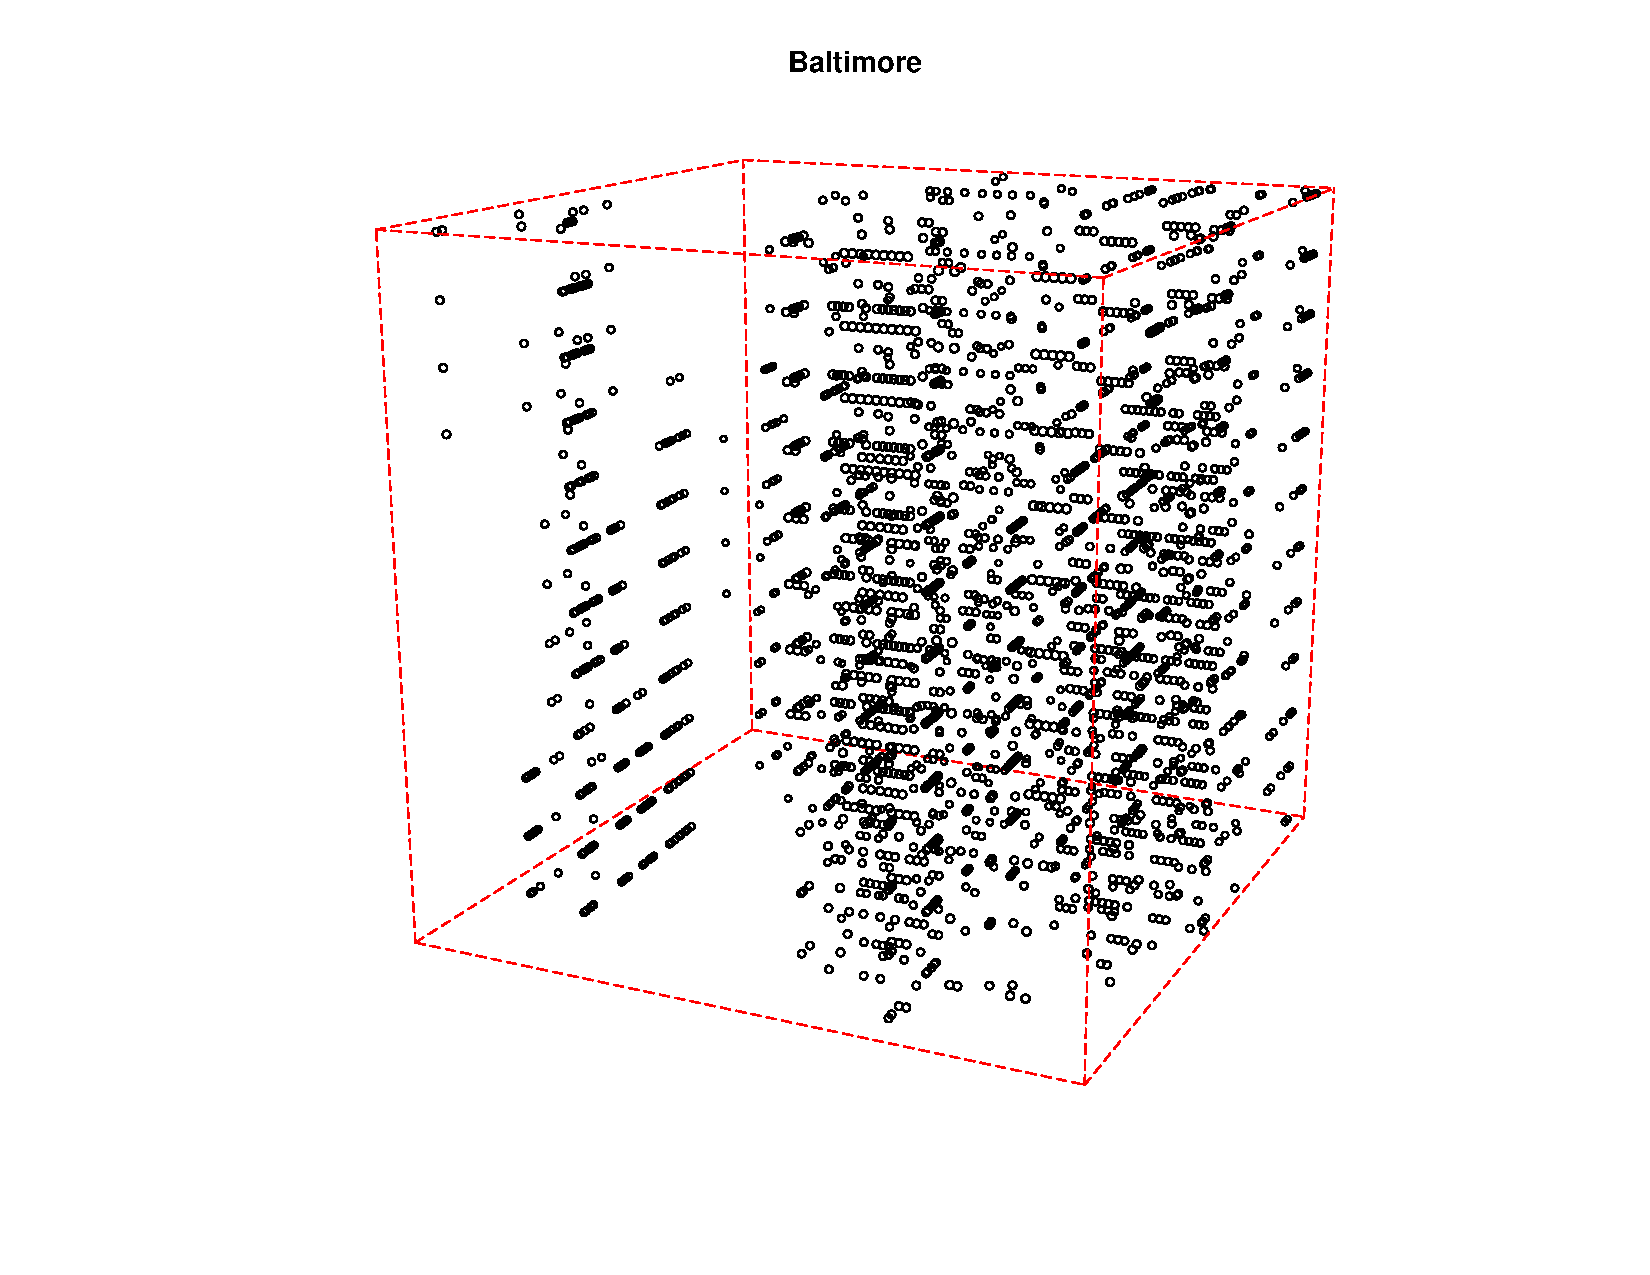
\includegraphics[width=0.9\textwidth]{PP_balt.pdf}
  \caption{Vacant flats represented as a spatio-temporal point process. First two dimension indicate location in coordinates, third dimension indicates year when flat was vacant. Number of points: 2538. }
  \label{fig:baltPP}

\vspace*{\floatsep}

    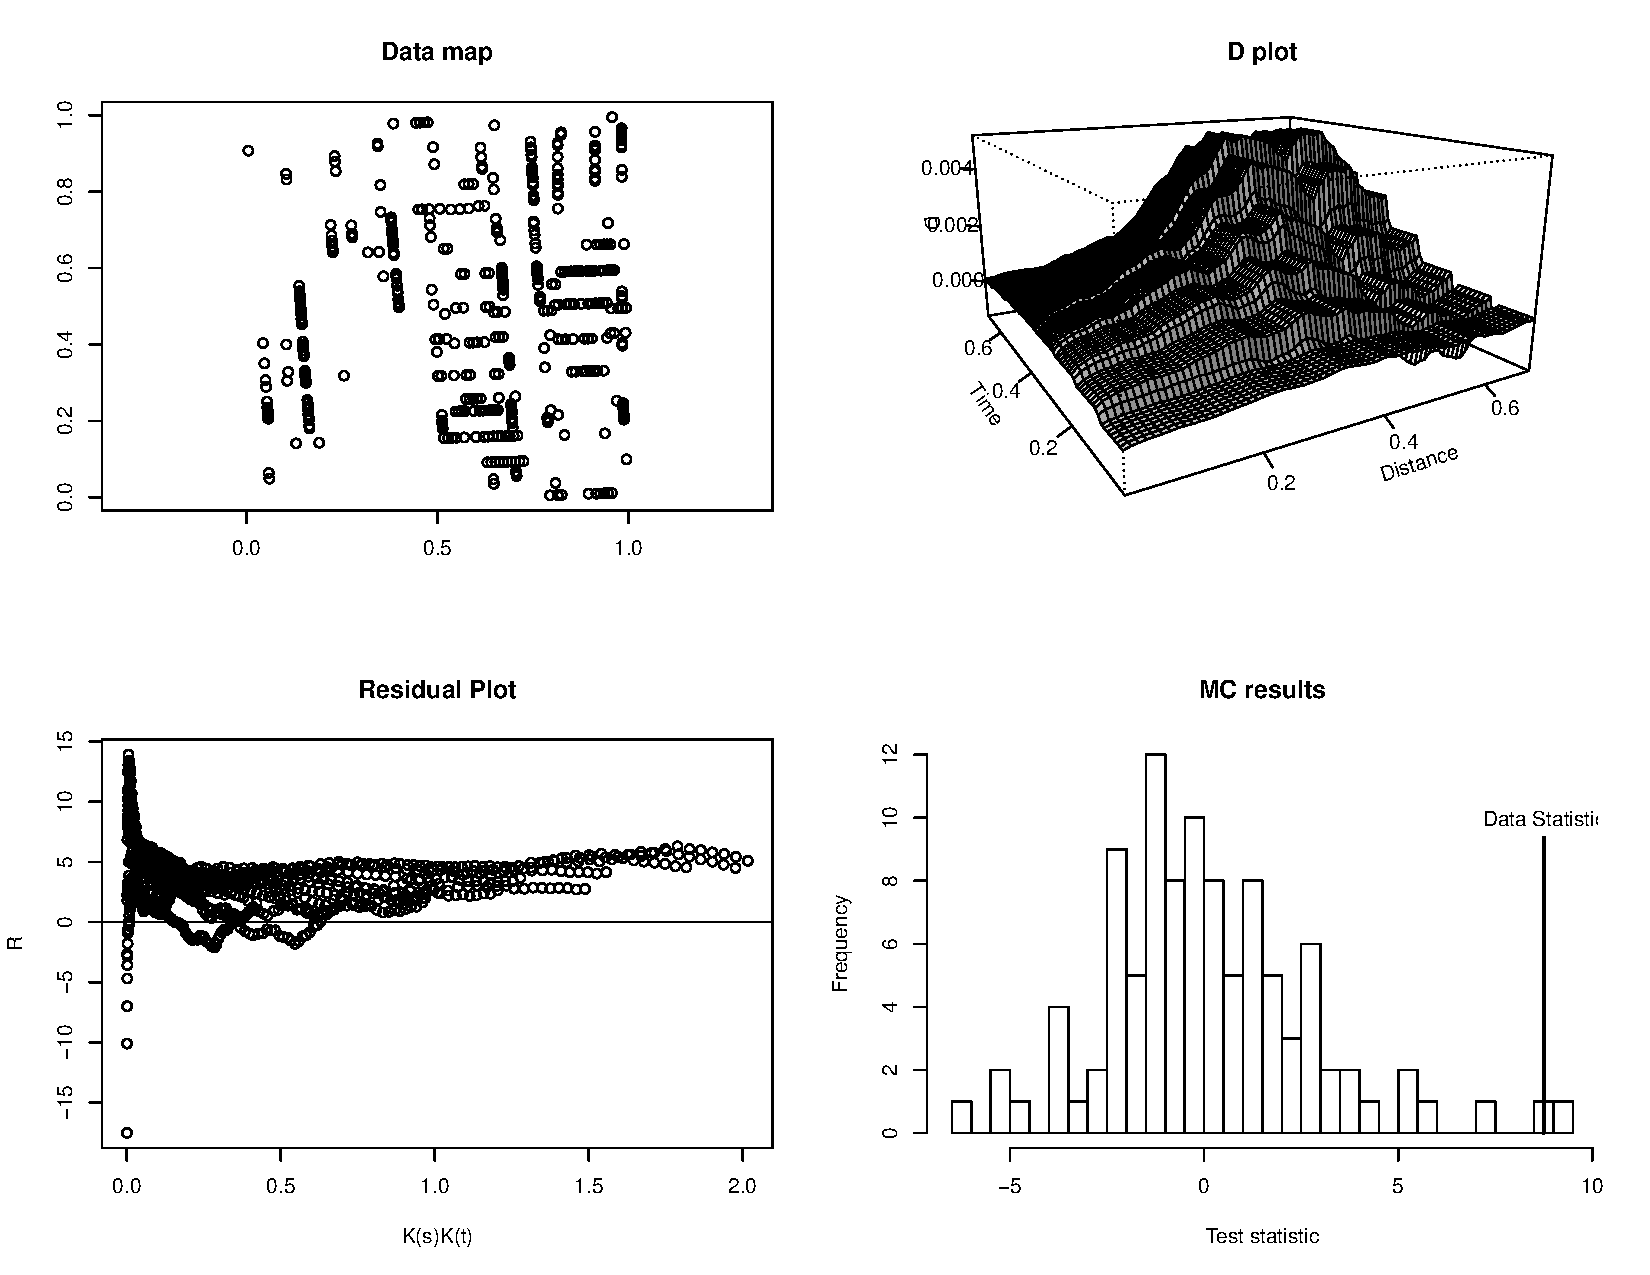
\includegraphics[width=0.9\textwidth]{diag_balt.pdf}
  \caption{Diagnostic plots for vacant flats represented as a spatio-temporal point process. Number of points: 2538. } 
  \label{fig:baltDiag}
\end{figure}



\begin{figure}[p]
  \centering
    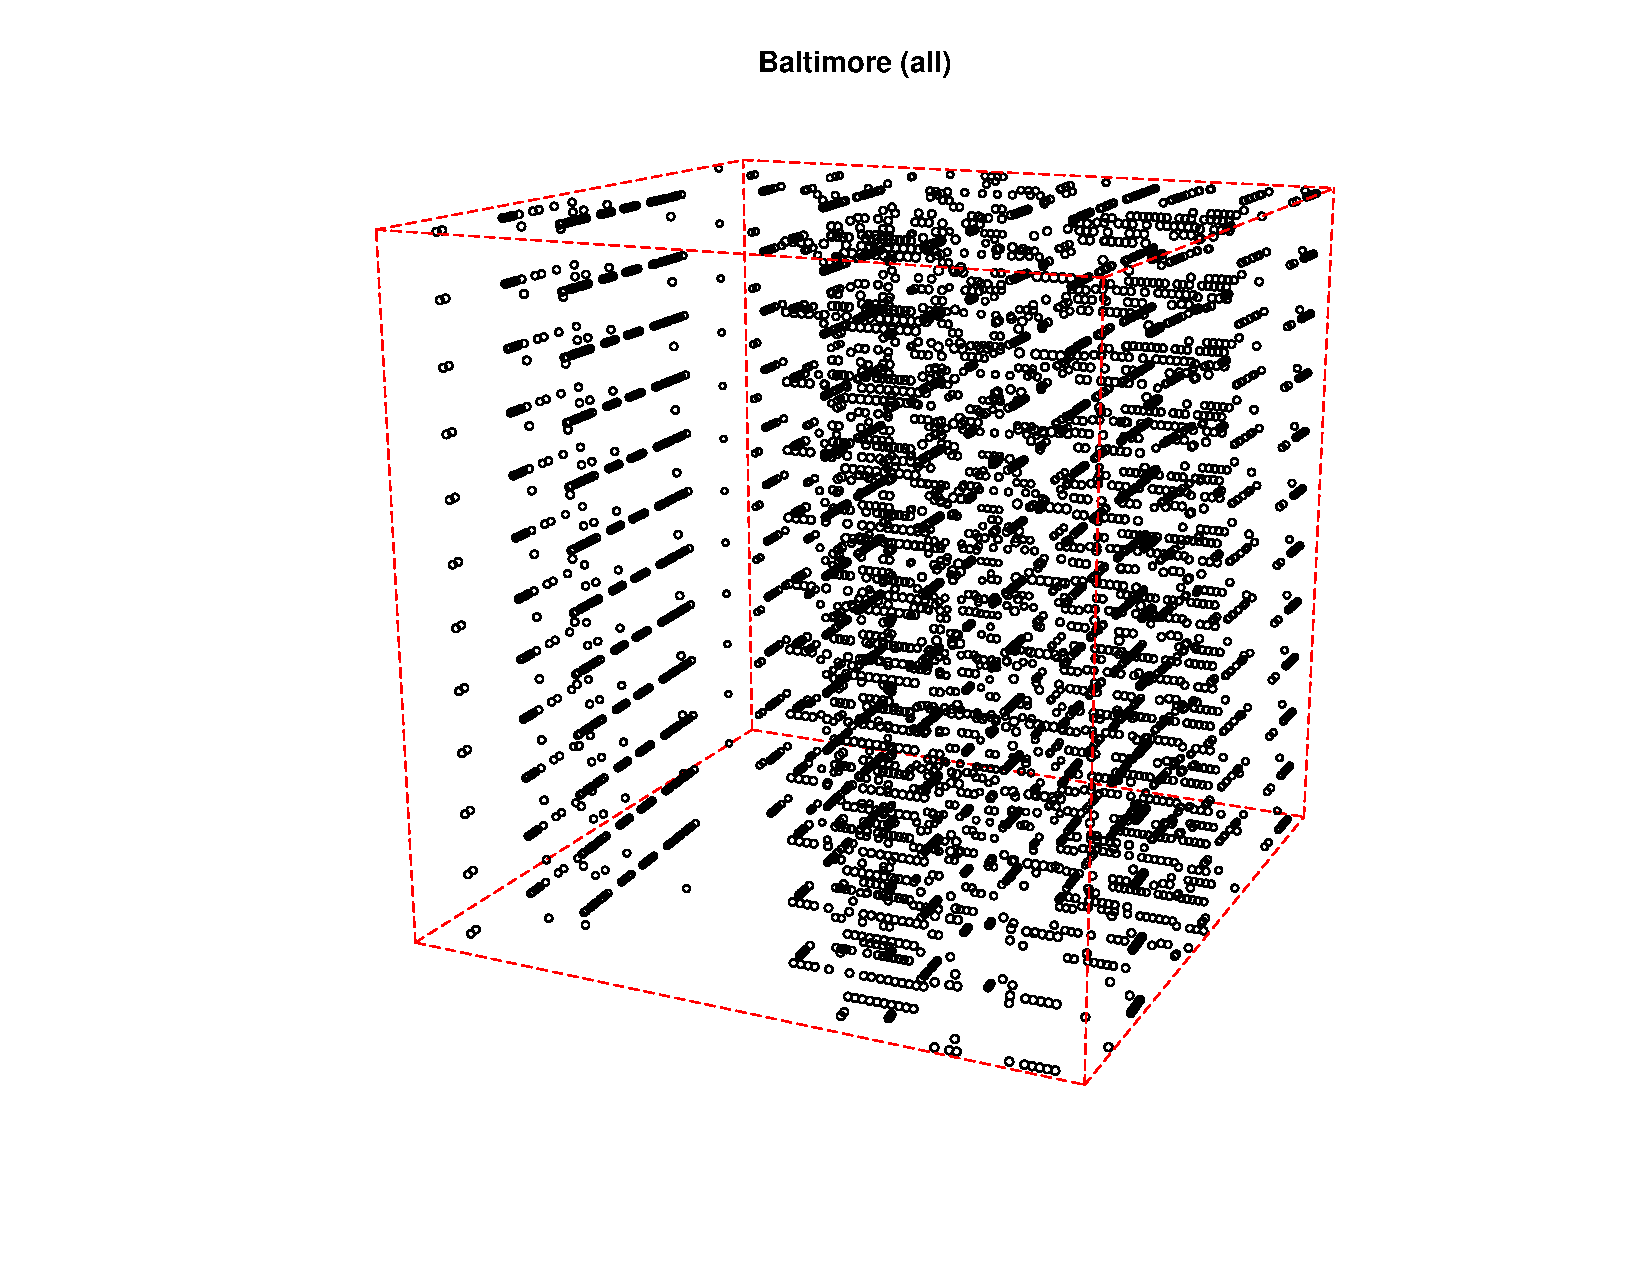
\includegraphics[width=0.9\textwidth]{PP_balt_full.pdf}
  \caption{Spatio-temporal point process composed of locations of all flats repeated in each year, regardless of whether it was vacant or not. Number of points: 4872. }
  \label{fig:baltallPP}

\vspace*{\floatsep}

    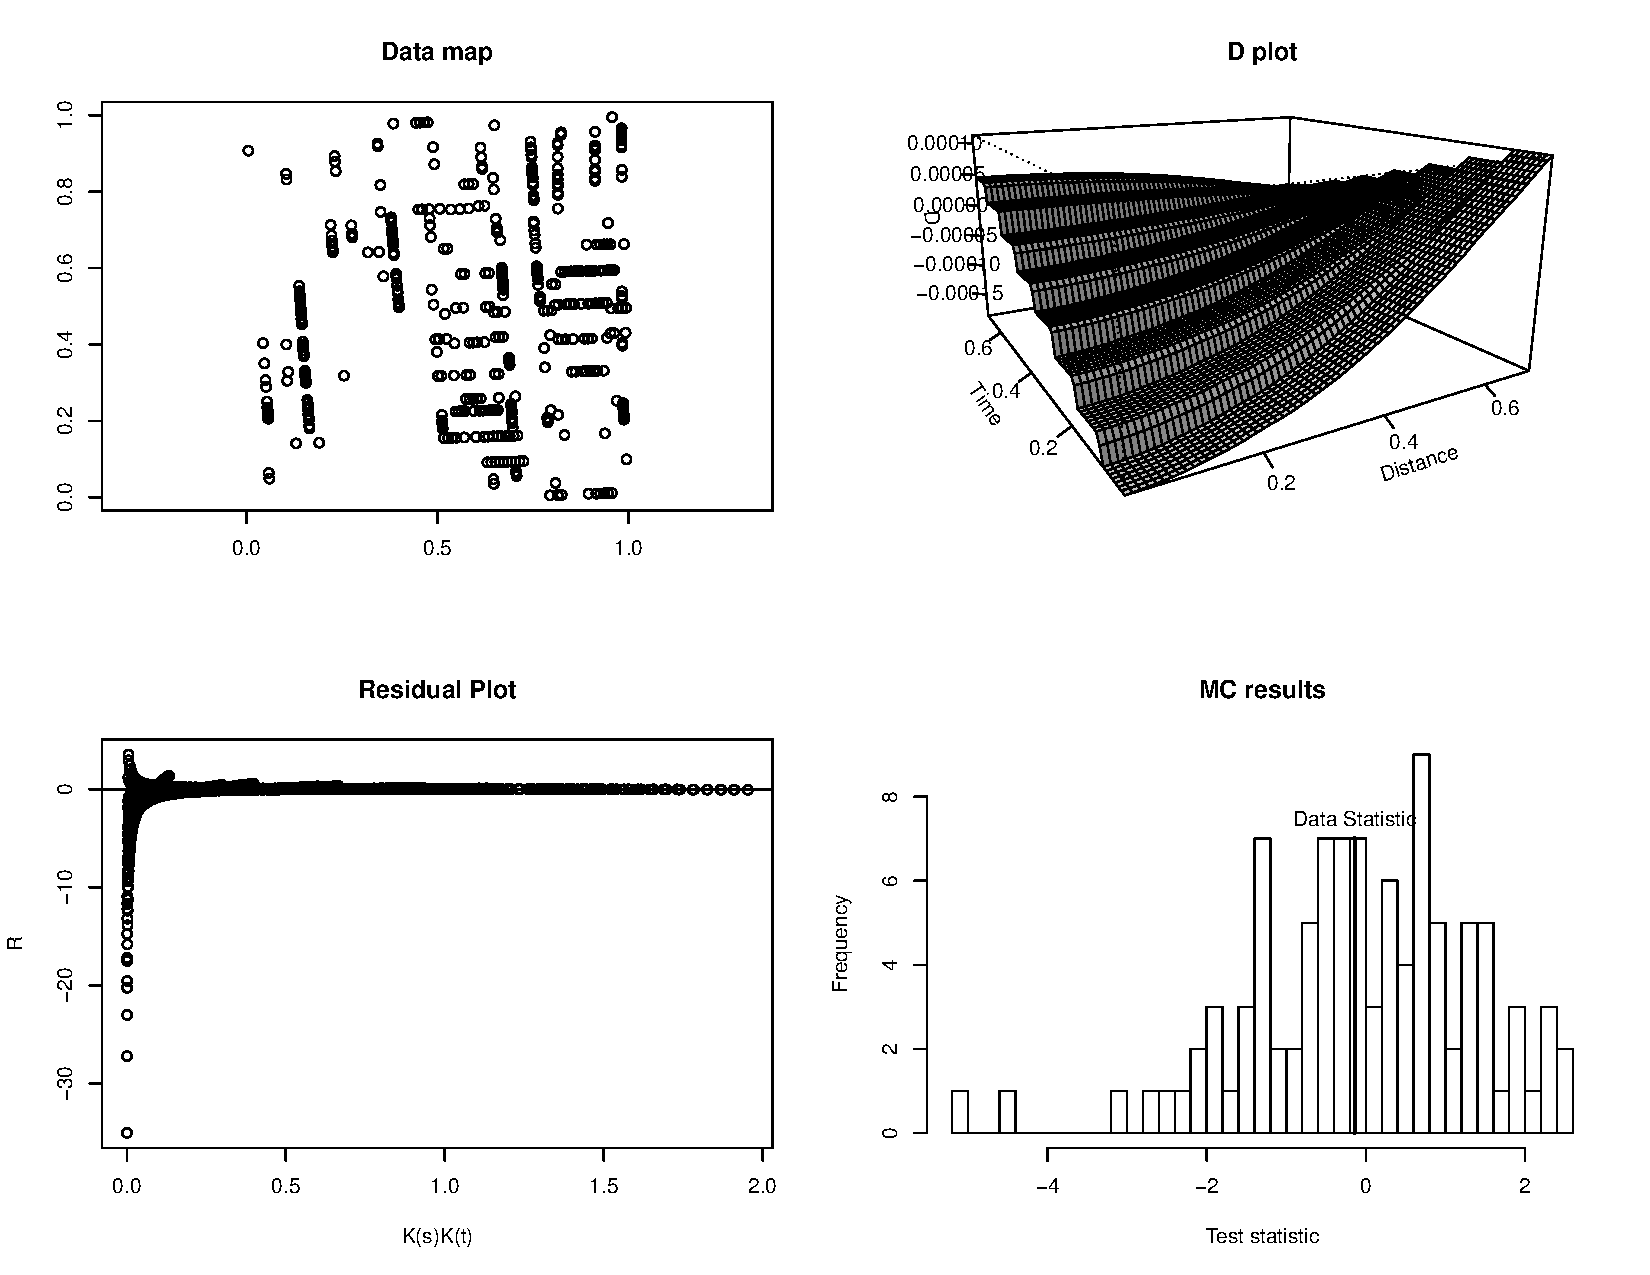
\includegraphics[width=0.9\textwidth]{diag_balt_full.pdf}
  \caption{Diagnostic plots for repeated locations of flats. Number of points: 4872. } 
  \label{fig:baltallDiag}
\end{figure}







\bibliography{bibliography}



\end{document}  %End of document.
